\begin{titlepage}

\begin{center}

%% Extra whitespace at the top.
\vspace*{2\bigskipamount}

%% Print the title.
\begin{spacing}{1.6}
{\makeatletter
\titlestyle\bfseries\LARGE\@title
\makeatother}
\end{spacing}

%% Print the optional subtitle.
{\makeatletter
\ifx\@subtitle\undefined\else
    \bigskip
    \titlefont\titleshape\Large\@subtitle
\fi
\makeatother}

\end{center}

\cleardoublepage
\thispagestyle{empty}

\begin{center}

%% The following lines repeat the previous page exactly.

\vspace*{2\bigskipamount}

%% Print the title.
\begin{spacing}{1.6}
{\makeatletter
\titlestyle\bfseries\LARGE\@title
\makeatother}
\end{spacing}

%% Print the optional subtitle.
{\makeatletter
\ifx\@subtitle\undefined\else
    \bigskip
    \titlefont\titleshape\Large\@subtitle
\fi
\makeatother}

%% Uncomment the following lines to insert a vertically centered picture into
%% the title page.
%\vfill
%\includegraphics{title}
\vfill

%% Apart from the names and dates, the following text is dictated by the
%% promotieregelement.

{\Large\titlefont\bfseries Proefschrift}

\bigskip
\bigskip

ter verkrijging van de graad van doctor

aan de Technische Universiteit Delft,

op gezag van de Rector Magnificus prof.~dr.~ir.~T.H.J.J.~van~der~Hagen,

voorzitter van het College voor Promoties,

in het openbaar te verdedigen

op woensdag 16 juni 2021 om 17:30 uur

\bigskip
\bigskip

door

\bigskip
\bigskip

%% Print the full name of the author.
\makeatletter
{\Large\titlefont\bfseries\@firstname\ \titleshape{\MakeUppercase{\@lastname}}}
\makeatother

\bigskip
\bigskip

Master of Science in Computer Science, \\
Technische Universiteit Delft, Nederland,

geboren te Sint-Maartensdijk, Nederland.

%% Extra whitespace at the bottom.
\vspace*{2\bigskipamount}

\end{center}

\clearpage
\thispagestyle{empty}

%% The following line is dictated by the promotieregelement.
\noindent Dit proefschrift is goedgekeurd door de

%% List the promotors (supervisors).
\medskip\noindent
\begin{tabular}{l}
    promotor: Prof.dr.ir.\ D.H.J.\ Epema \\
    promotor: Dr.ir.\ J.A.\ Pouwelse
\end{tabular}

\bigskip
\noindent Samenstelling promotiecommissie:

%% List the committee members, starting with the Rector Magnificus and the
%% promotor(s) and ending with the reserve members.
\medskip\noindent
\begin{tabular}{p{4.5cm}l}
    Rector Magnificus, & voorzitter \\
    Prof.dr.ir.\ D.H.J. Epema, & Technische Universiteit Delft, promotor\\
    Dr.ir.\ J.A. Pouwelse, & Technische Universiteit Delft, promotor\\

    \medskip
    \mbox{\emph{Onafhankelijke leden:}} & \\
    Prof.dr.\ A. van Deursen, & Technische Universiteit Delft \\
    Prof.dr.\ A.-M. Kermarrec, & École polytechnique fédérale de Lausanne, Switzerland \\
    Prof.dr.\ F.\ Taïani, & Université de Rennes 1, France \\
    Dr.\ A.\ Gervais, & Imperial College London, United Kingdom \\
    Dr.\ D.G.J. Bongaerts, & Erasmus University Rotterdam \\
    
    Prof.dr.\ K.G. Langendoen & Technische Universiteit Delft, reservelid \\ \\

\end{tabular}

%% Include the following disclaimer for committee members who have contributed
%% to this dissertation. Its formulation is again dictated by the
%% promotieregelement.
%\medskip
%\noindent  %Prof.\ Dr.\ D.\ Spinellis has contributed to the creation of this thesis.

%\medskip
%\medskip
% TODO Include http://www.win.tue.nl/ipa/?page_id=309
%\noindent The work in the thesis has been carried out under the auspices of the research school ASCI (Advanced School for Computing and Imaging).

%\medskip
%% Here you can include the logos of any institute that contributed financially
%% to this dissertation.
\medskip
\begin{center}
    
\includegraphics[height=0.5in]{title/logos/tudelft}
    \hspace{4em}
    %
\includegraphics[height=0.5in]{title/logos/casimir} \\
%    
\includegraphics[height=0.5in]{title/logos/nwo}
%    \\ \vspace{0.5cm}
    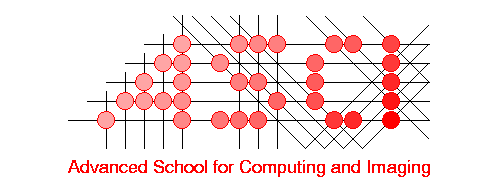
\includegraphics[height=0.55in]{title/logos/asci}
\end{center}
%\vfill
\medskip

\noindent This work was carried out in the ASCI graduate school.\\ASCI dissertation series number 420.


\vfill
\medskip
\medskip

\noindent
\begin{tabular}{@{}p{0.2\textwidth}@{}p{0.8\textwidth}}
  \textit{Keywords:} & decentralization, disintermediation, electronic markets, e-commerce, blockchain, decentralized exchanges, matchmaking, settlement, fraud, information management, identity management, decentralized finance, trading, money \\[\medskipamount]
      \textit{Printed by:} & Gildeprint B.V., Enschede, The Netherlands \\[\medskipamount]
      \textit{Cover by:} & Martijn de Vos and Jeannet Stoutjesdijk. The cover shows an artistic impression of a decentralized network.  \\[\medskipamount]
      \textit{Style:} & TU Delft House Style, with modifications by Moritz Beller \\& \url{https://github.com/Inventitech/phd-thesis-template} \\[\medskipamount]
\end{tabular}

\medskip
\medskip
\noindent The author set this thesis in \LaTeX\xspace using the Libertinus and Inconsolata fonts.

\vspace{\bigskipamount}

% Copyrighting this is stupid, questionable, and probably illegal, because large parts of the
% thesis have already been published with the copyright resigning with the publisher.
%\noindent Copyright \textcopyright\ 2015 by A.~Einstein

%% Uncomment the following lines if this dissertation is part of the Casimir PhD
%% Series, or a similar research school.
%\medskip
%\noindent Casimir PhD Series, Delft-Leiden 2015-01

%\medskip
\noindent ISBN \todo{TBD}

\medskip
\noindent An electronic version of this dissertation is available at \\
\url{http://repository.tudelft.nl/}.

\end{titlepage}

